\chapter{The relationship between perception and production}\label{ch:Perception-Production}

In the models examined to this point, the tokens of perception have
been assumed to be identical to the tokens of production. This assumption
obscures the fact that targets in production are necessary in order
for sounds to be produced at all, i.e., that read-out of a stored
set of acoustic values is not possible. It also conflates biases that
act in production with those that act in perception, requiring them
to act on the same units. Furthermore, this assumption requires that
complex articulatory dynamics be uniquely and transparently realized
acoustically. For a dimension like segment duration, this assumption
may not be too unreasonable. However, the correspondence between articulation
and acoustics is well known to be a many-to-many mapping. Invariant
cues to abstract phonemes have failed to be discovered in either domain. 

Starting at least with \citet{Goldinger1996}, it has been assumed
that experienced exemplars are stored as motor plans without intermediate
processing. While this may be adopted largely as an implementational
convenience, it is based on the assumption that the true details of
the mapping will not significantly affect the mechanism of change,
or the model outcomes (see \citealt{Pierrehumbert2000}). Perhaps
the most critical assumption is that they will not affect the feedback
loop that is the driving mechanism of such models. However, as this
chapter will demonstrate, a non-trivial perception-to-production mapping
is not just an additive factor that can be slotted into existing models,
but a shift in perspective that affects all aspects of modeling, up
to and including what we take to be the source of sound change itself.
The following sections will make these ramifications explicit for
three cases representing three different types of phonetic bias (two
of which have been previously modeled): vowel lengthening (duration-based
targets); vowel nasalization (sequencing of different articulators);
and velar palatalization (sequencing of different targets for the
same articulator). 

\section{Duration-based targets}

The lack of motivation for a process by which a production, at some
random point along the relevant dimension, is moved only a small amount
towards its target, was mentioned briefly in \sectref{sec:Model-Interpretation}.
Failure to completely achieve a target may not seem paradoxical at
first glance, because it suggests a well-known articulatory phenomenon,
known as “undershoot”, in which targets fail to be completely
achieved (e.g. \citealt{Lindblom1963}). But this is not an equivalent
process.\footnote{The centering bias in \citet{Wedel2008} is characterized as a lenition
bias towards the center of each segment dimension. Because Wedel's
categories lack underlying targets (they are randomly generated and
evolve as poor, or ambiguous, tokens are discarded), his lenition
bias is the mechanism that prevents categories from dispersing indefinitely.
For a two-dimensional phonetic vowel space composed of the first and
second formant frequencies, a centralizing bias is fairly consistent
with undershoot. However, this bias is implemented as a fixed attractor
location, rather than a process that shifts the vowel formants a small
amount towards the center of formant space on each production. This
suggests that there is a target, or ideal, vowel location from which
all vowels are perturbed by other forces. }

Undershoot can occur if over-all speech rate is rapid, not allowing
enough time to overcome the inertia inherent in the physical articulators,
or if sequential targets involving the same articulator (e.g. tongue
body) are far apart in the mouth. A duration target, however, cannot
be undershot in the same way. In the first place, segment duration
\emph{per se} is not specified on individual articulators or their
configurations. Furthermore, duration is not absolute. Thus, although
a faster speaking rate will lead to shorter vowel durations, it will
also shorten all segments in all contexts, meaning that the relative
difference between vowel durations in pre-voiced versus pre-voiceless
contexts will not necessarily be affected (unless duration values
are at floor or ceiling). A speaking rate transformation effectively
changes the location of the target itself in absolute terms; it does
not affect the speaker's ability to reach that target for any given
token. Length-based features are arguably better modeled by targets
that are a function of speaking rate. 

With respect to the effect of frequency on duration, the mechanism,
and its interaction with speaking rate, remains somewhat unclear.
In models of frequency effects, speaking rate does not seem to be
considered. Yet the parallels between the two are clear. The conceptualization
of frequency of use as repeated practice suggests that there exists
a maximally fluent, or optimal, production target. While increased
frequency should not reduce any word below that target, increased
speaking rate might. If frequency of use translates to higher resting
activation, on the other hand, and higher resting activation leads
to faster production, successive shortening should only occur if listeners
fail to normalize for speaking rate; and if they fail to normalize
for speaking rate, then the stored distribution will reflect the typical
variance in speaking rate. This issue will be taken up in Chapter
\ref{ch:Phoneme-Split}, with two different implementations of the
frequency effect.

\section{Coordination of independent articulators}

In the vowel nasalization example of \sectref{subsec:Model-3:-Nasalization}
it was assumed that nasalization occurred when a given vowel token
was produced adjacent to a nasal consonant, transforming from completely
oral ($[-nasal]$), to completely nasal ($[+nasal${]}). This simulation
was useful for illustrating the context mismatch that would result
from nasalized tokens being produced in a non-nasal context (which
occurs whether nasality is considered binary or not). Our current
purpose, however, is to consider how an articulatory phenomenon like
nasality could be modeled iteratively with the classic perception-production
loop. 

In most exemplar models ``phonetic bias'' is taken to apply without
limit, and without regard to input values. That is, lengthening will
occur regardless of how long the vowel already is, provided it occurs
in a pre-voiced context. For the phenomenon of vowel nasalization
this requires some partial nasalization that applies whenever a vowel
is produced preceding a nasal consonant, a partial nasalization that
is additive in nature. This is schematized in (\ref{Ex: Iterative Nasality}). 
\begin{covexample}
\label{Ex: Iterative Nasality}$\textit{Nasalization}(V)\rightarrow V^{+N}$

$\textit{Nasalization}(V^{+N})\rightarrow V^{+2N}$

$\textit{Nasalization}(V^{+2N})\rightarrow V^{+3N}$
\end{covexample}
But this type of acoustic cumulativity is only possible under a very
specific, and unlikely, production model. 

As first described in \sectref{subsec:Model-3:-Nasalization},
phonetic vowel nasalization is the product of the coarticulation that
occurs throughout normal speech. Sounds are not produced in strict
sequence but overlap considerably with their neighbors. In the case
of a vowel-nasal sequence, the velum, or soft palate, is raised in
anticipation of the nasal segment before the vowel gesture has completed,
resulting in airflow through the nasal cavity during at least part
of the vowel's production. To represent the articulatory side of this
phenomenon, and draw a clear distinction between perceived tokens
and their correspondents in production, we will make use of the representational
tools of Articulatory Phonology (AP) (\citealt{Browman1986,Browman1990}). 

In AP, the abstract representational units of speech are taken to
be analogous to musical scores, which indicate the coordination and
ordering of a series of physical movements (articulatory gestures).
Those gestures involve a set of active articulators – the tongue,
velum, glottis, etc. – usually in relation to a set of passive articulator
locations – the teeth, lips, hard palate, etc. Scores consist of a
series of target locations for each active articulator (e.g. the
alveolar ridge behind the teeth), and timing relations between those
movements (e.g. begin movement of tongue tip at midpoint of open
glottis gesture). \figref{fig:Normal nasalization} depicts a gestural
score for nasal coarticulation, based on the specific sequence {/æm/}.
Time is represented along the x-axis, and the active articulators
are shown on the y-axis (TB=Tongue Body; VEL=velum). The box adjacent
to each active articulator represents the time span during which that
articulator is activated: gradually moving towards it target position,
then away to a subsequent target, or resting state. The interval during
which the boxes overlap indicates the period when the two articulators
are active at the same time. This overlap, indicated by the space
between the dotted lines in \figref{fig:Normal nasalization}, is
the source of the vowel nasalization of interest. 

\begin{figure}[H]
\begin{subfigure}[t]{.3\textwidth}
        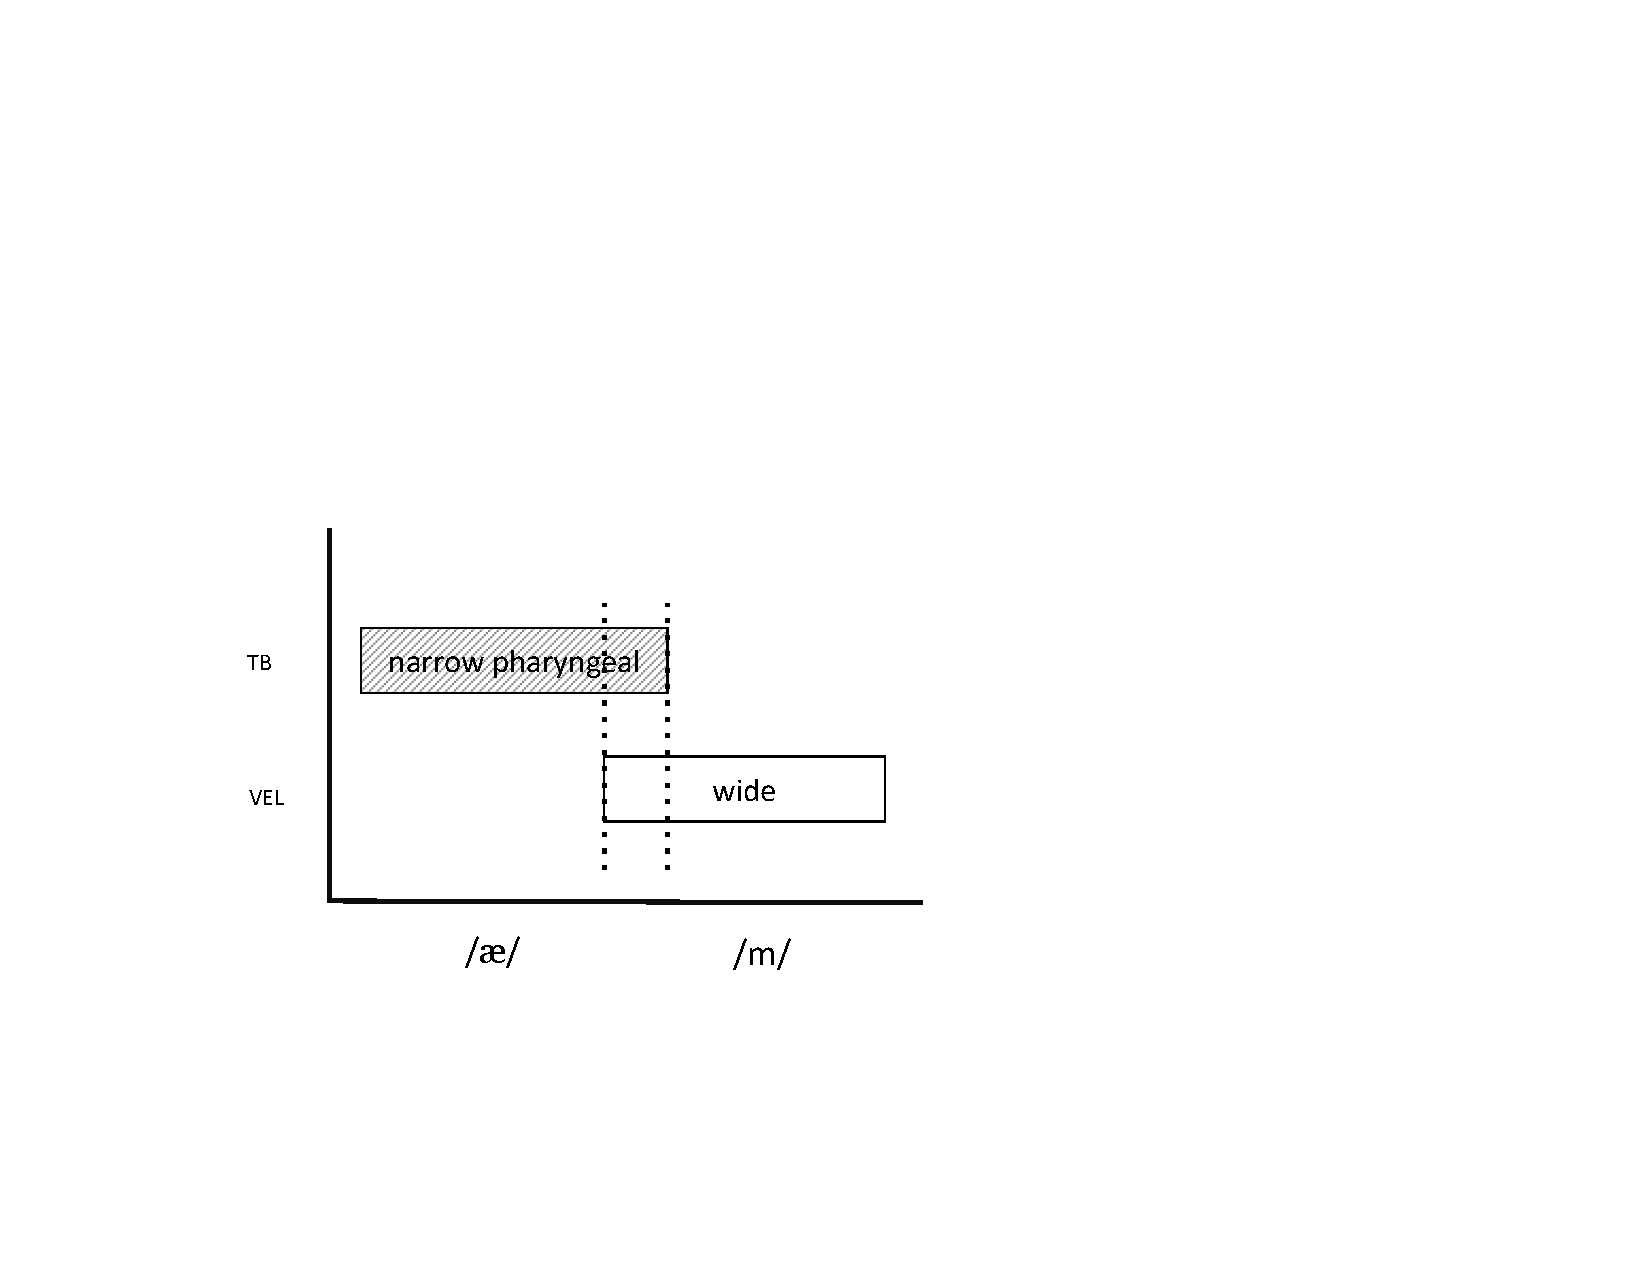
\includegraphics[width=\linewidth]{figures/nasalization1.pdf}
        \caption{\label{fig:Normal nasalization}Nasalization of underlyingly oral vowel token}
    \end{subfigure}\hfill
    \begin{subfigure}[t]{.3\textwidth}
        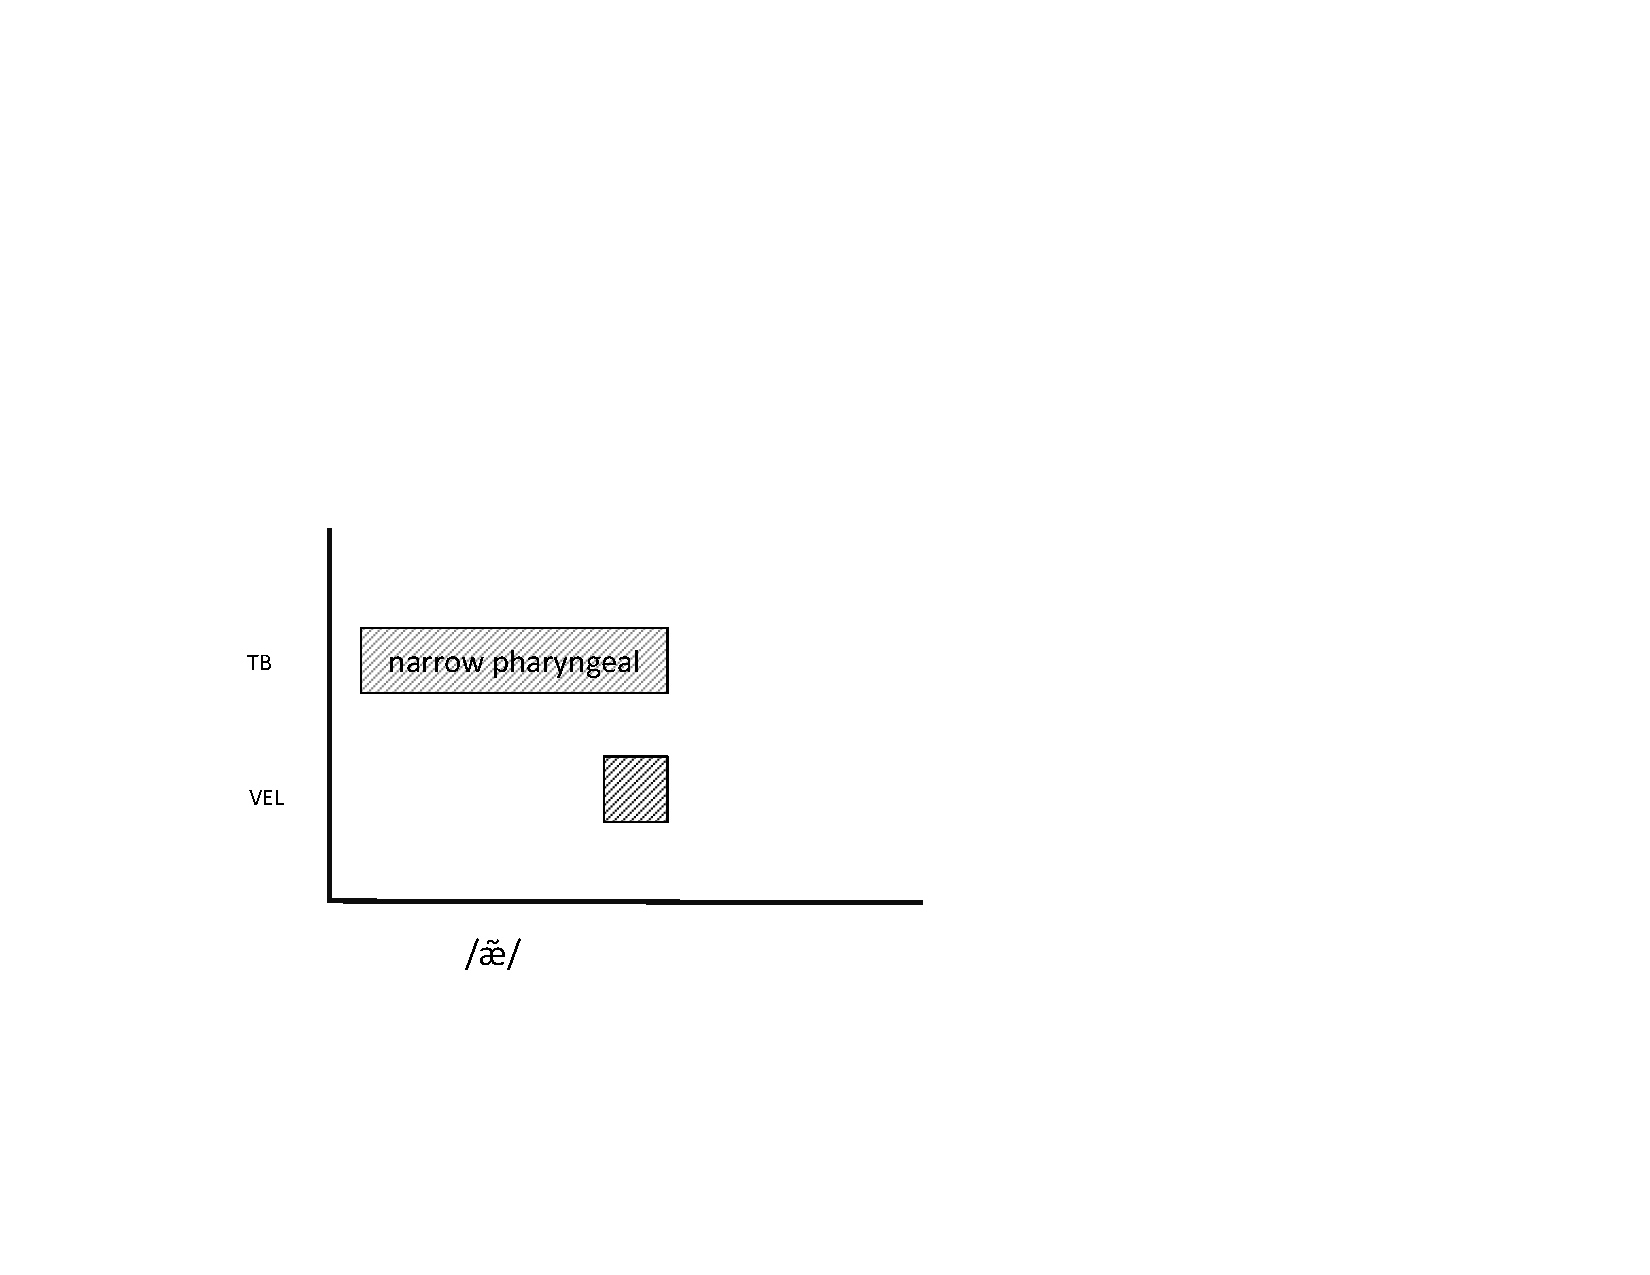
\includegraphics[width=\linewidth]{figures/nasalization2.pdf}
        \caption{\label{fig:nasalized vowel}Underlyingly nasalized vowel token (unnormalized)}
    \end{subfigure}\hfill
    \begin{subfigure}[t]{.3\textwidth}
        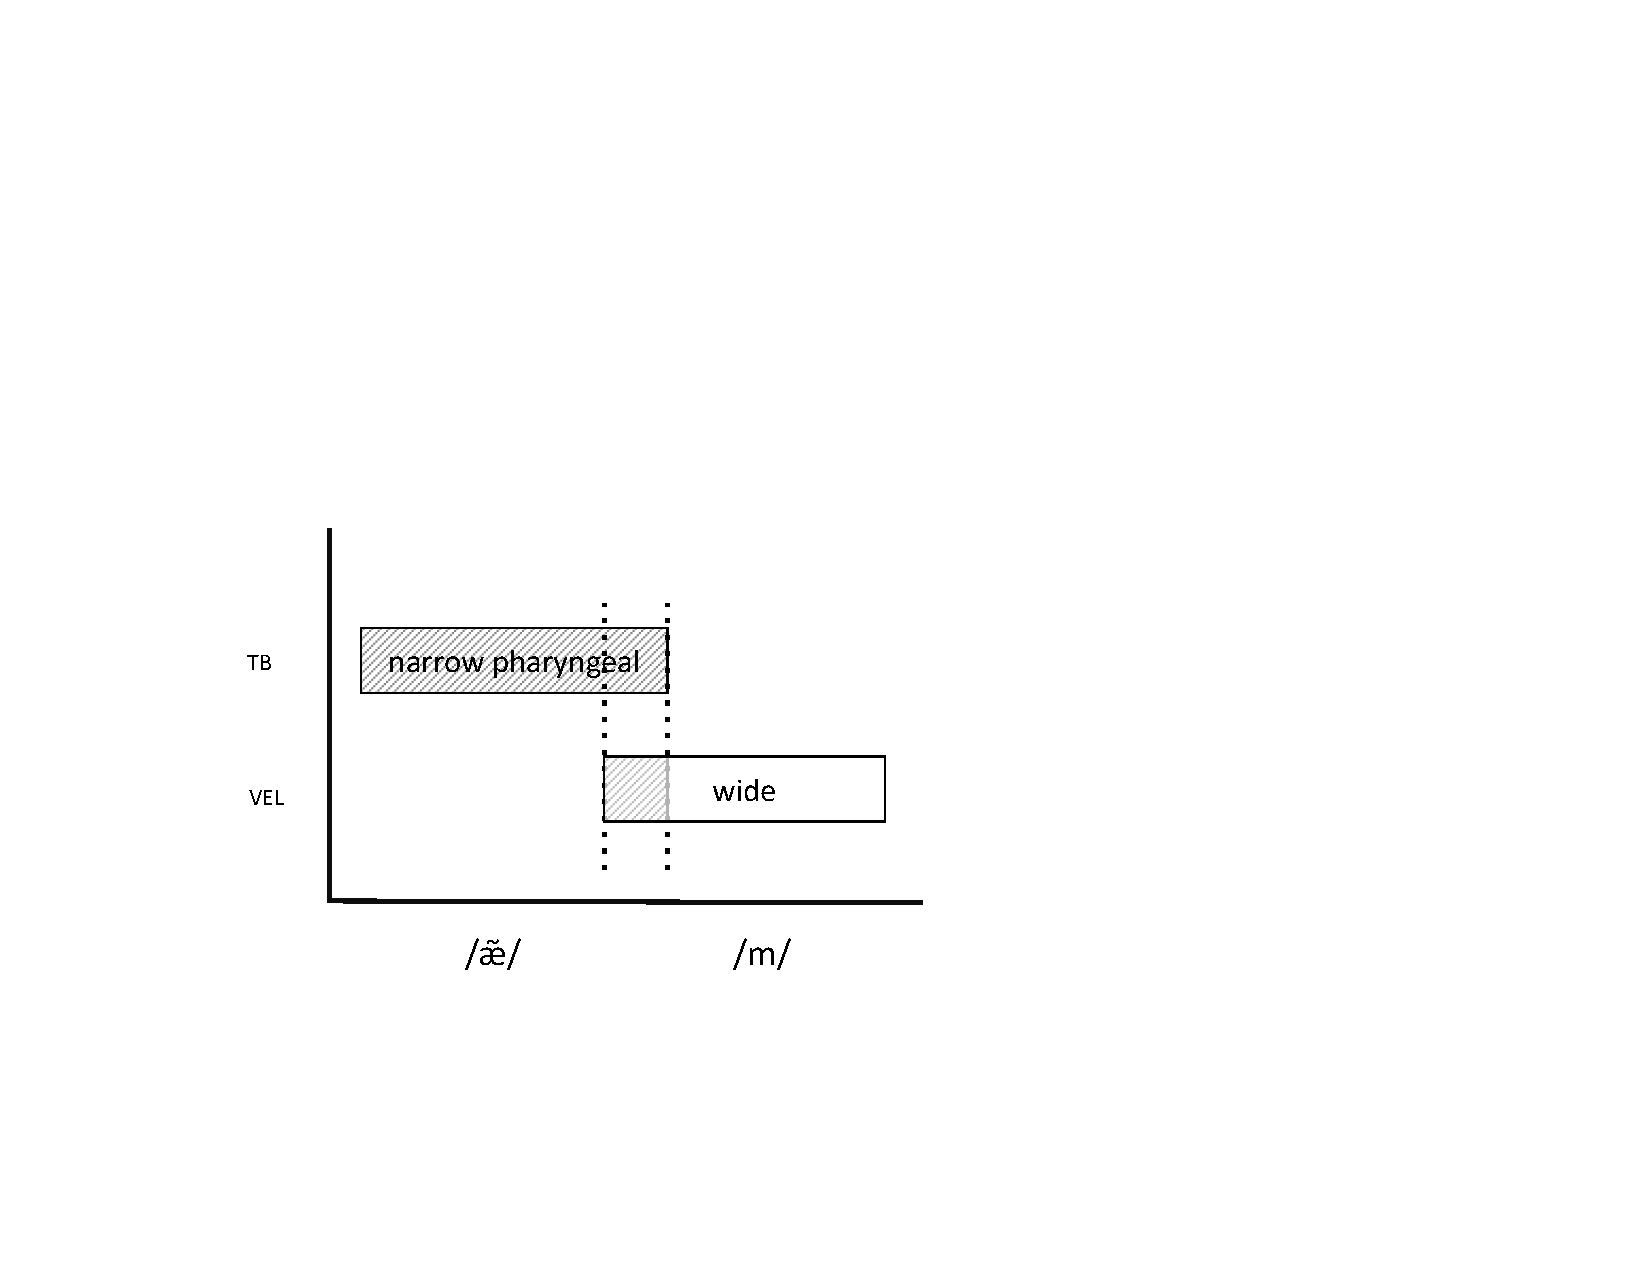
\includegraphics[width=\linewidth]{figures/nasalization3.pdf}
        \caption{\label{fig:extra nasalization}Nasalization of underlyingly nasal vowel token}
    \end{subfigure}
    
% % \subfloat[\label{fig:Normal nasalization}Nasalization of underlyingly oral
% % vowel token ]{\includegraphics[width=0.25\textwidth]{figures/nasalization̘1.pdf}}\hfill{}\subfloat[\label{fig:nasalized vowel}Underlyingly nasalized vowel token (unnormalized)]{\includegraphics[width=0.25\textwidth]{figures/nasalization̘2.pdf}}\hfill{}\subfloat[\label{fig:extra nasalization}Nasalization of underlyingly nasal
% % vowel token]{\includegraphics[width=0.25\textwidth]{figures/nasalization̘3.pdf}}

\caption{\label{fig:Coarticulation}Coarticulation involving different articulators}
\end{figure}

The gestural score indicated in \figref{fig:Normal nasalization}
produces the acoustic realization {[æ̃m]}. The vocalic
portion of this token, if stored without normalization, is represented
by {/æ̃/}. The two different types of brackets are used
here in exactly their usual sense: square brackets indicate a surface
form, an instance of speech, while forward slashes indicate an underlying
form, a form used to generate a speech act. Before such an acoustic
token can be produced, however, it must be converted to an articulatory
representation. This is shown in \figref{fig:nasalized vowel}.
Note that, despite the fact that the nasalization is now a property
of the vowel itself, the same two articulatory gestures are still
required in production.

At some still later model cycle, when the token represented in (\ref{fig:nasalized vowel})
is chosen for production in the identical nasal context, the combined
articulatory score is realized as \figref{fig:extra nasalization}.
Under error-free perception and production, the velum gesture associated
with the vowel (indicated by diagonal fill lines), and the velum gesture
associated with the nasal will overlap completely. And because there
is only one velum, there will be only one velum gesture. Acoustically,
this will result in exactly the same amount of nasality on the vowel
as before ({[æ̃]}). The feedback loop is, in fact, halted
after a single iteration. The only way that the vowel could become
successively more nasalized is if the velum were to begin raising
earlier and earlier in time – in other words, if a successive change
in the timing relationship were to occur.\footnote{Differences in the amount of velar opening and degree of velar airflow
can be found among different types of nasalized vowels (\citealt{bell1993understanding,hajek2000vowel}).
But this is a property of a given vowel. There is no reason for the
greater degree of velar opening for a low vowel, for example, to be
increased further each time that vowel is produced preceding a nasal.} But a change of this nature requires independent motivation. In
other words, the iterative result does not come for free when the
acoustic-articulatory mapping is no longer an identity relation. 

\section{\label{sec:Competing-targets}Competing targets for the same articulator}

The final case of perception-to-production mapping considered here
is one that contains conflicting consecutive specifications for a
single articulator. A common phenomenon of this type is palatalization,
which involves the tongue shifting towards the hard palate (either
forward or backward) due to the influence of a following or preceding
segment (\citealt{Guion1998,Keating1993}). Palatalization often occurs
in sequences of obstruent consonants and high vowels. For example,
in the articulation of the sequence {/ki/}, the articulatory
target of the {/k/} is the velum, or soft palate, where the
tongue body makes contact, briefly creating a complete closure in
the oral cavity. The articulatory target for the vowel is closer to
the hard palate, where the tongue body should reach its highest point,
but without making contact. As a result of the upcoming tongue body
specification for the {/i/}, the tongue position for the
{/k/} is shifted forwards – away from the soft palate, and
towards the hard palate. The result is a “blend”, something
that is in between where the two gestures would be in isolation (\citealt{Browman1986,Zsiga2000}). 

The blended production for the palatalized velar is depicted in \figref{fig:/k+i}. 
At the bottom of the figure, the boxes represent
temporal extent as before, this time of the single Tongue Body articulator.
Diagonal fill lines represent the duration when the {/k/}
target is active, and the semi-opaque white, the duration of the active
{/i/} articulation. Above, the trajectory of the highest
point of the tongue body relative to the two target locations is indicated
by the dotted line. The tongue body is assumed to start from a resting
position that places its highest point somewhere in between the hard
and soft palates. With the start of the {/k/} gesture, movement
of the tongue body is initiated towards the soft palate. However,
because the gesture of the following {/i/} is anticipated,
a shift in direction takes place before this target is reached, causing
both targets to be only partially achieved (the solid curves indicate
the target trajectories for each segment in isolation). 

\begin{figure}[H]

\begin{subfigure}[t]{.50\textwidth}
        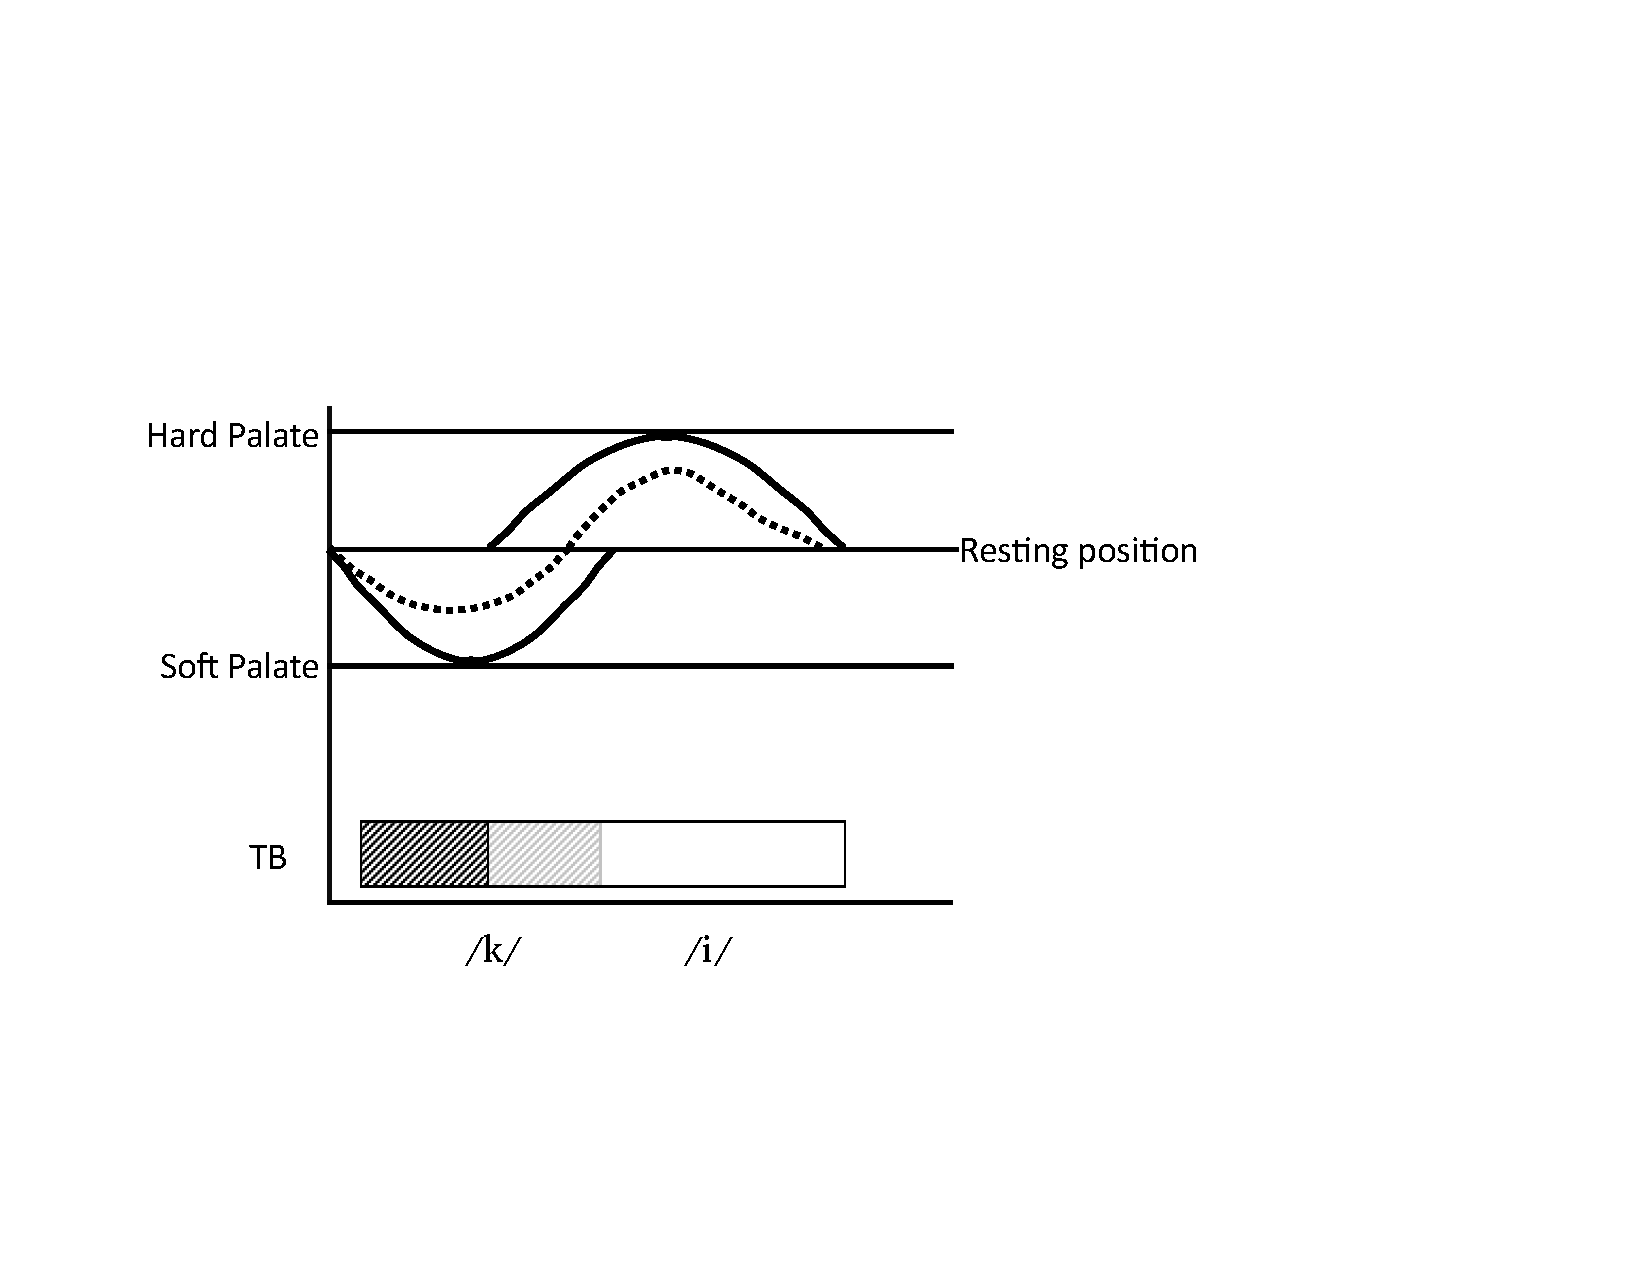
\includegraphics[width=\linewidth]{figures/palatalizationa.pdf}
        \caption{\label{fig:/k+i}/k+i/}
    \end{subfigure}\hfill
    \begin{subfigure}[t]{.50\textwidth}
        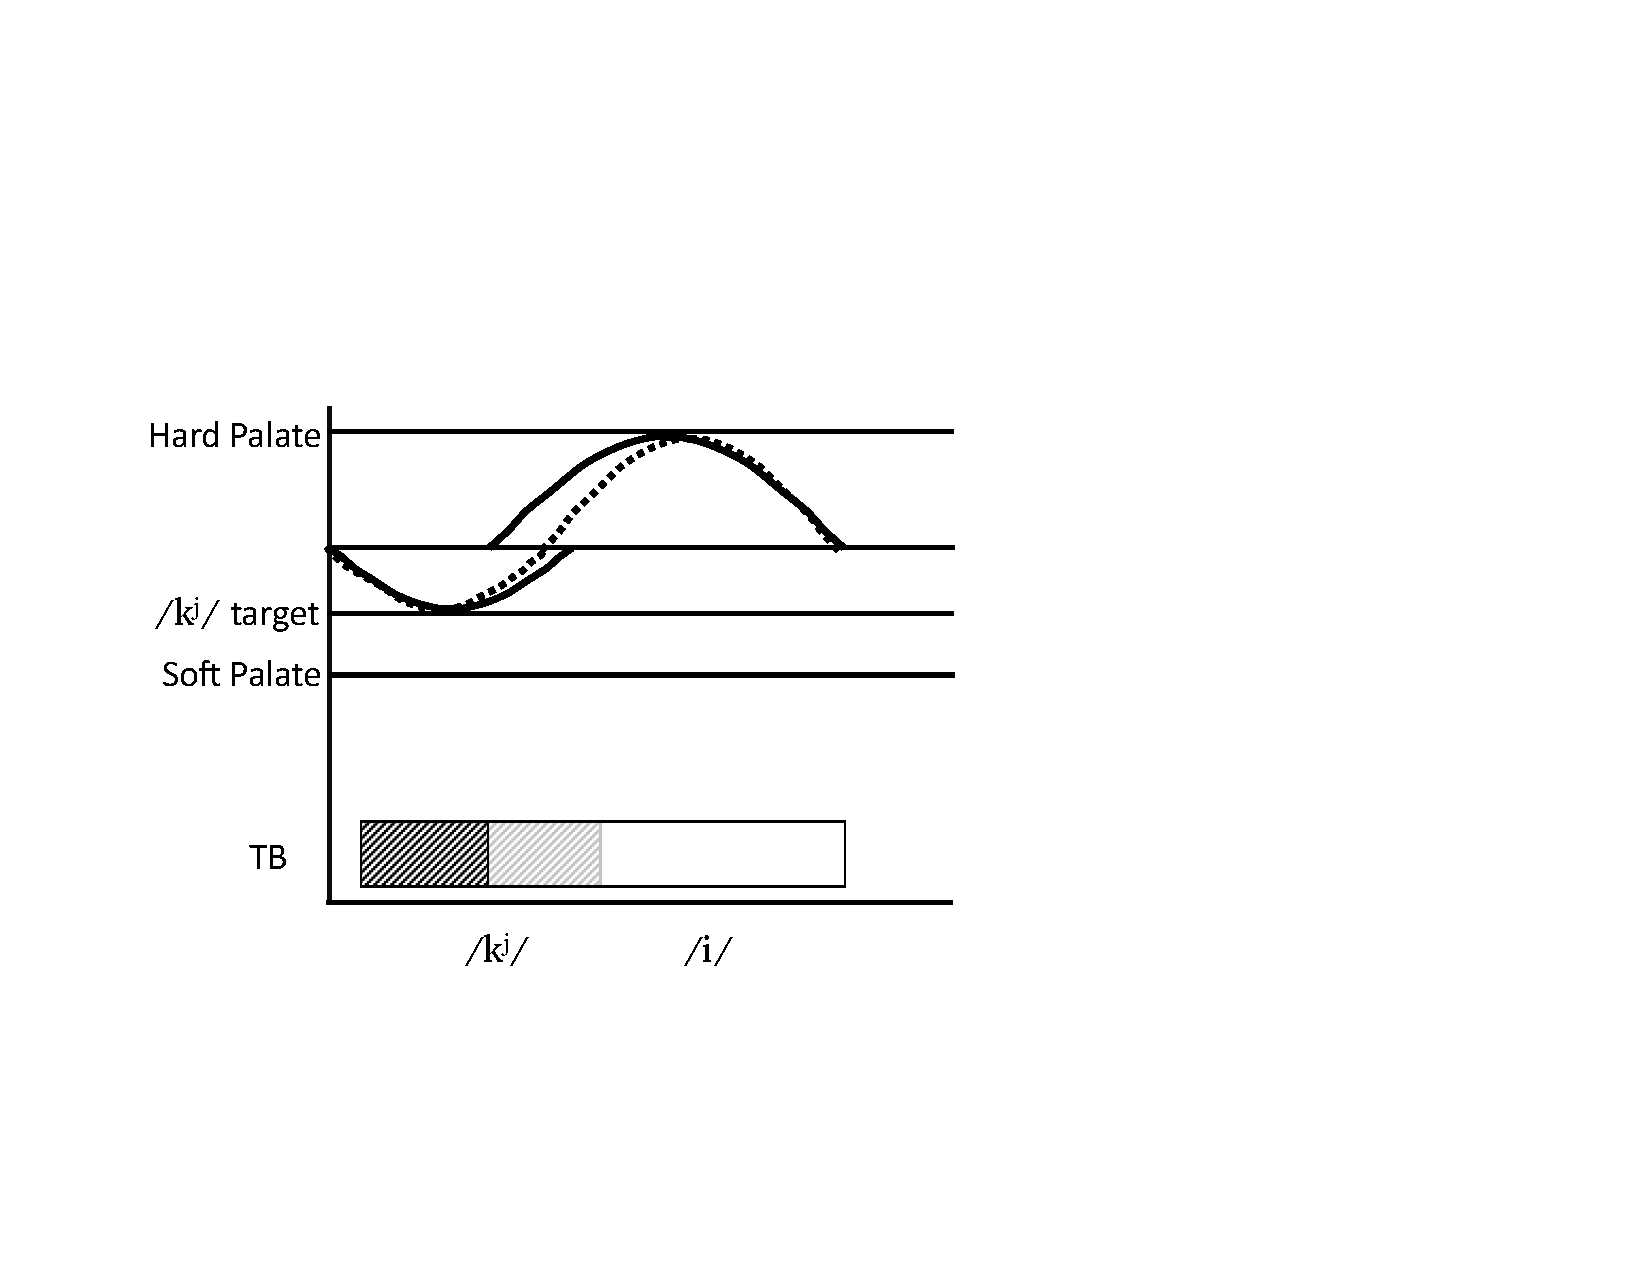
\includegraphics[width=\linewidth]{figures/palatalizationb.pdf}
        \caption{\label{fig:/k=0002B2+i/} {/kʲ+i/}}
    \end{subfigure}
    
    
% % \subfloat[\label{fig:/k+i}/k+i/]{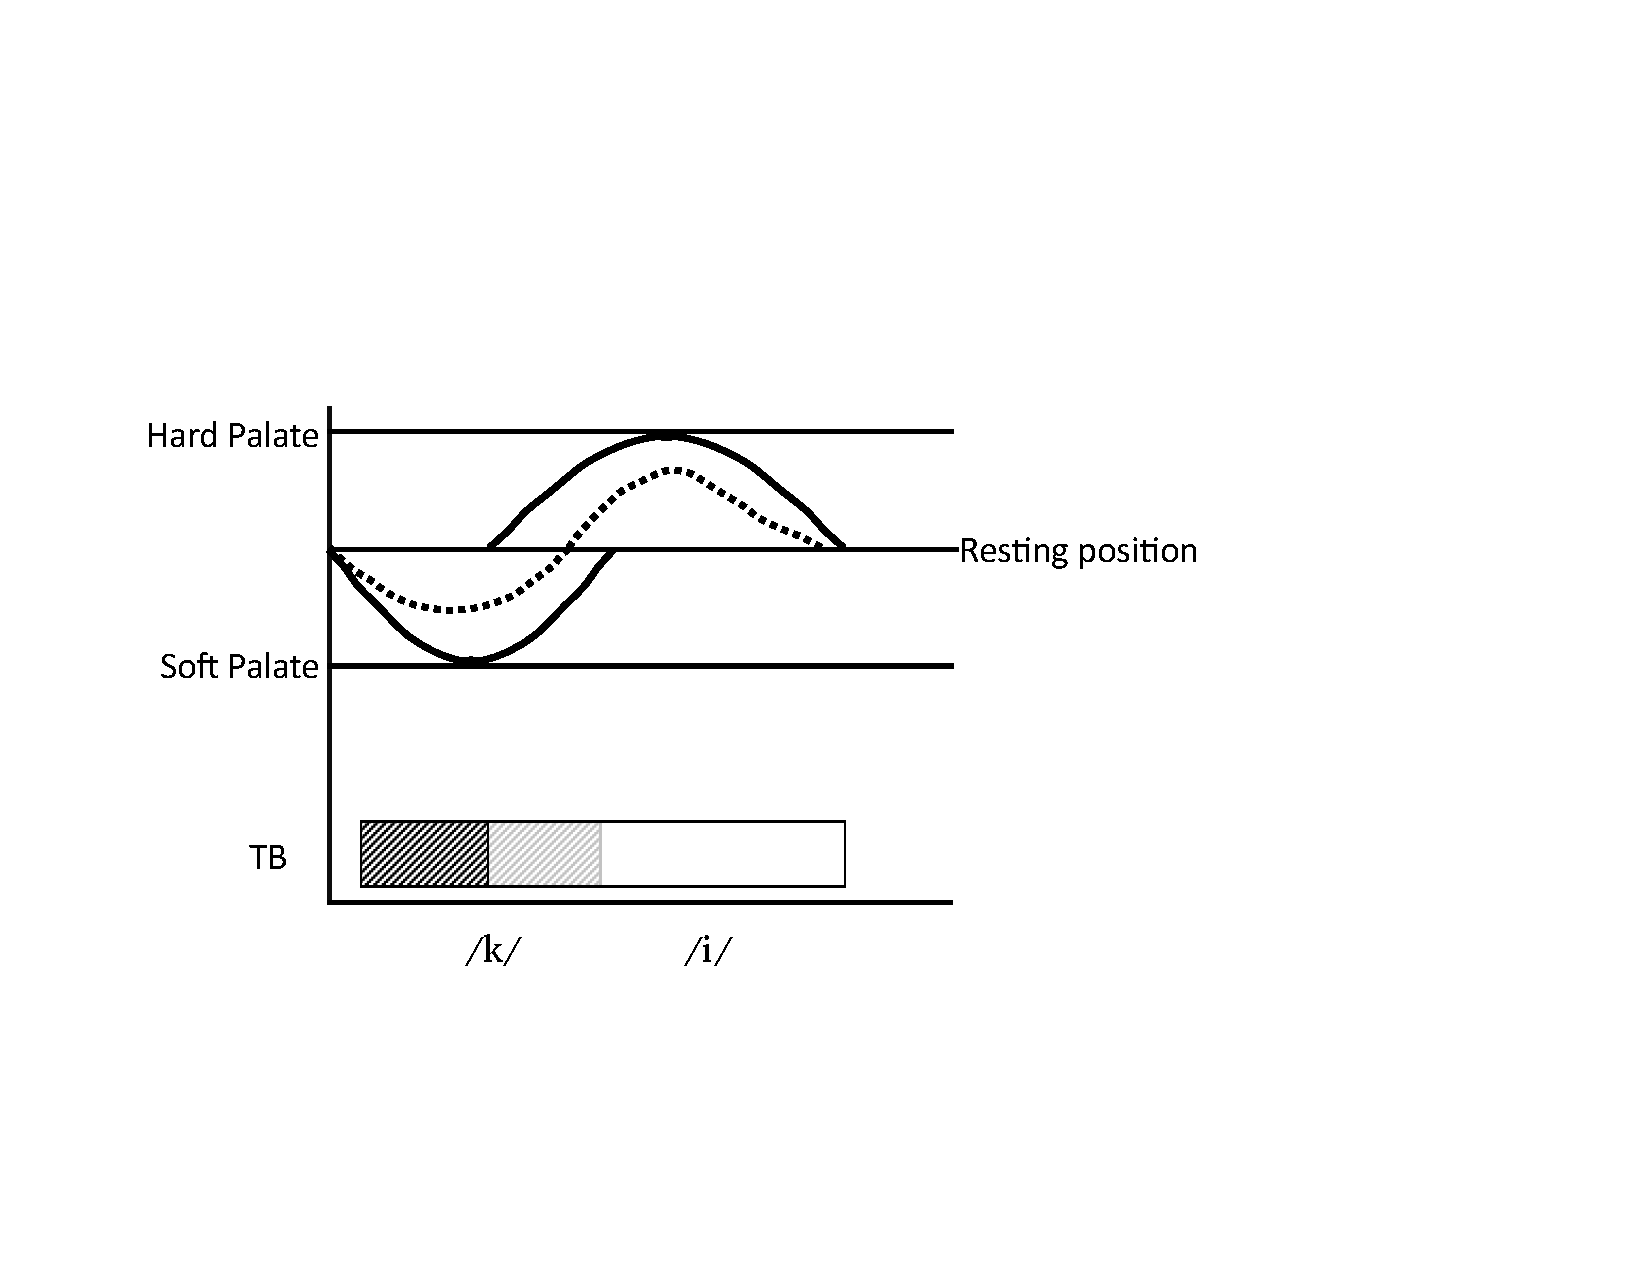
\includegraphics[width=0.4\textwidth]{figures/palatalizationa.pdf}}\hfill{}\subfloat[\label{fig:/k=0002B2+i/} {/kʲ+i/}]{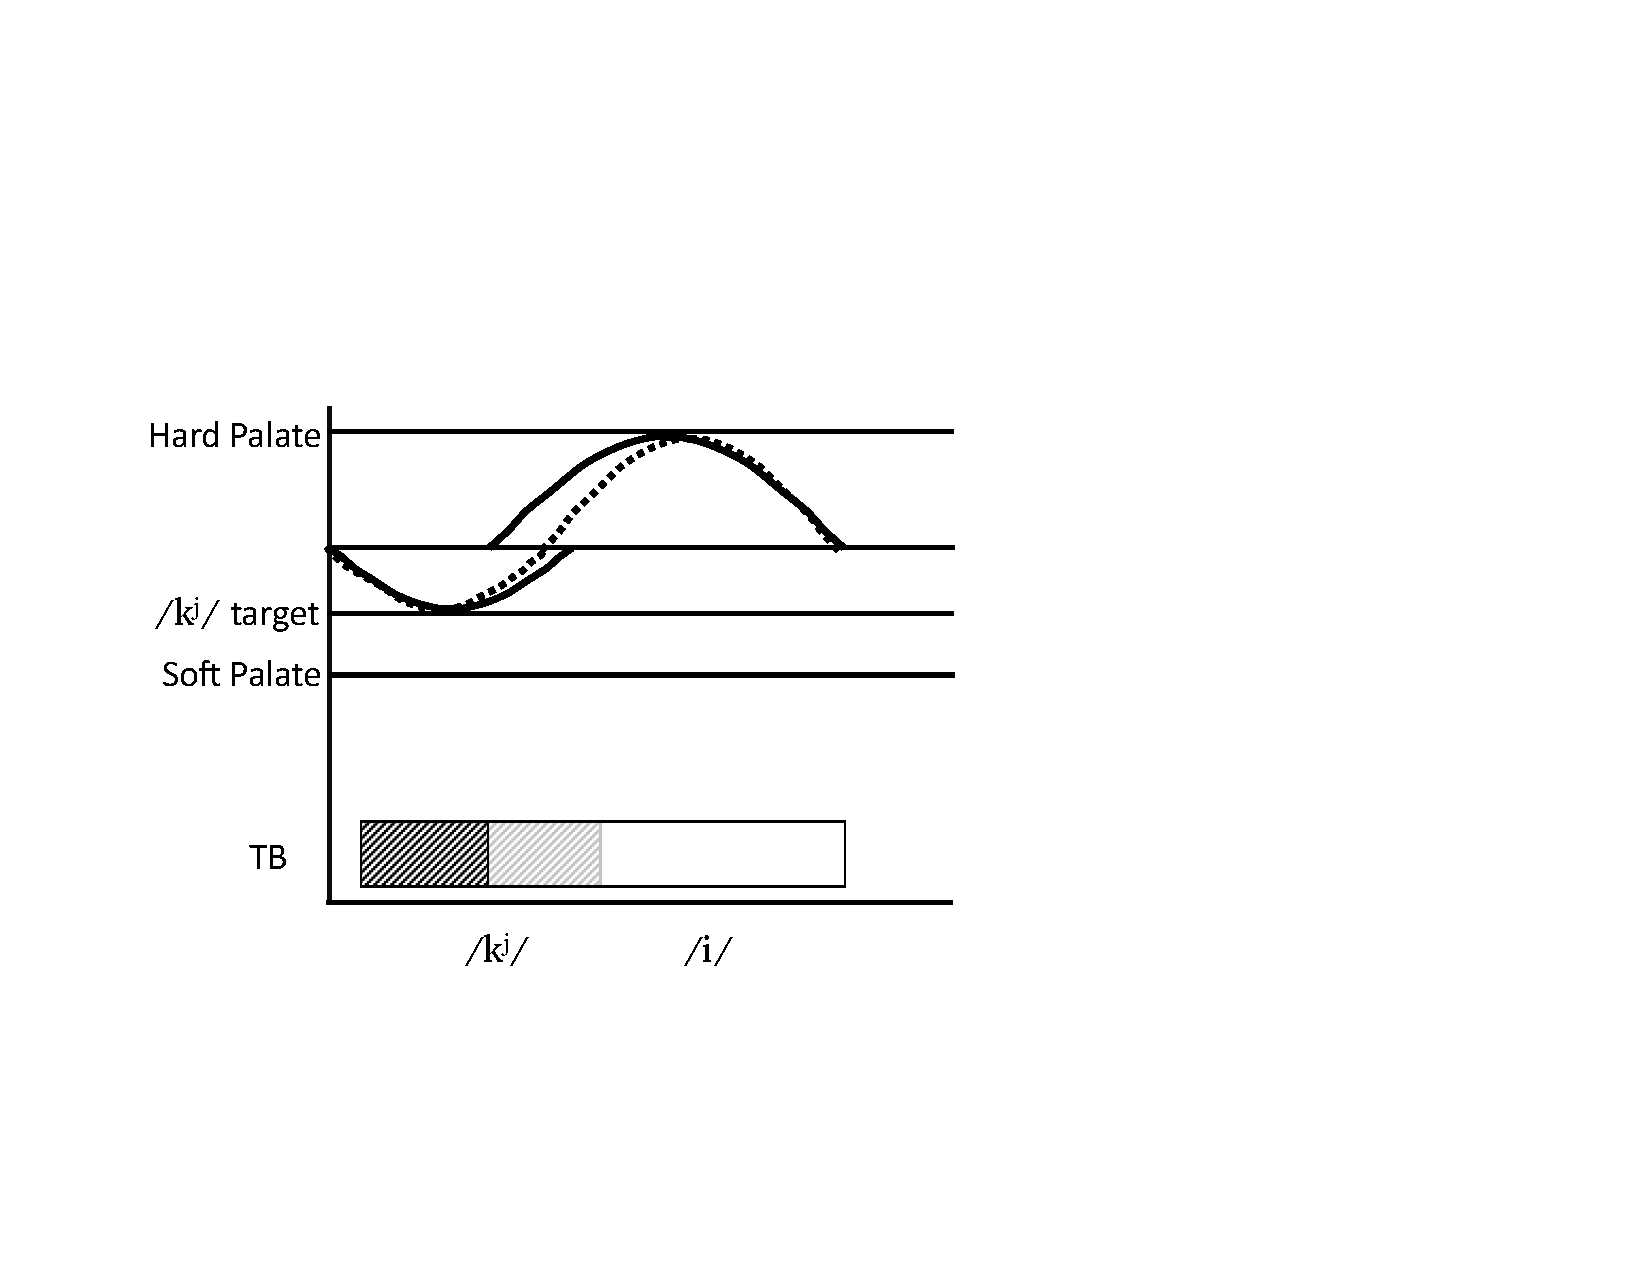
\includegraphics[width=0.4\textwidth]{figures/palatalizationb.pdf}}

\caption{Coarticulation involving the same articulator. The dark solid lines
represent the trajectories of each segment in isolation. The dotted
line represents the actual trajectory. The Tongue Body (TB) is taken
to start and finish in a resting position in between the two targets. }
\end{figure}

We will take the acoustic counterpart to this production token to
correspond to a sequence of partially palatalized velar and high front vowel, {[kʲ]}, {[i]}. The articulatory representation associated with the acoustic
representation {/kʲ/} contains a TB gesture located at the
minimum of the dotted curve in \figref{fig:/k+i}. On a subsequent
production cycle in which this token is produced in the context of
a following {/i/} ({/kʲ+i/}), the “palatalizing
bias” will result in something like the dotted curve in \figref{fig:/k=0002B2+i/}.
Effectively, the strength of the bias has been reduced. This is because
the amount of bias depends on the distance between the two targets,
and the target of the {/kʲ/} is closer to the target of
the {/i/}. In fact, it may now be possible to reach both
targets via a slight modification in the gestural timing. In other
words, there is no clear necessity of (continuously) shifting the
target location for the obstruent closer to the hard palate, resulting
in successively more palatalized tokens. 

There is actually more than one plausible acoustic interpretation
of the output of \figref{fig:/k+i}, and thus more than one articulatory
mapping for tokens derived from the original production of the {/k+i/}
sequence. The target locations of both the consonant and the vowel
may be altered, or the perceived boundary between the two segments
may be shifted, or both. \figref{fig:Palatalizationc} depicts a
scenario in which the entire sequence has been stored as an exemplar
of the original {/k/} category: a composite segment consisting
of two sequenced targets.\footnote{Using the IPA to represent acoustic correspondents is not ideal, due
not only to the conflation of acoustic and articulatory information,
but because it is not fine-grained enough to capture all the relevant
differences among the gestural scores. The composite analysis could
alternatively be represented as {/kʲ/} (as opposed to the
original {/kʲ/+/i/}). A change in both targets might look
like {/kʲ/+/ɪ/}. Other possibilities include: {/k/+/j/+/i/},
{/k/+/j/}, {/k͡j/}.} This particular type of mapping is of considerable interest because
it is not structure-preserving at the phoneme level. If the perception-to-production mapping itself is the cause of the loss or the
gain of a phoneme, then phoneme split may be possible without an independent
change that eliminates conditioning context – it may, in fact, follow
directly from a merger of the allophone with the allophonic context. 

\begin{figure}[H]
\centering{}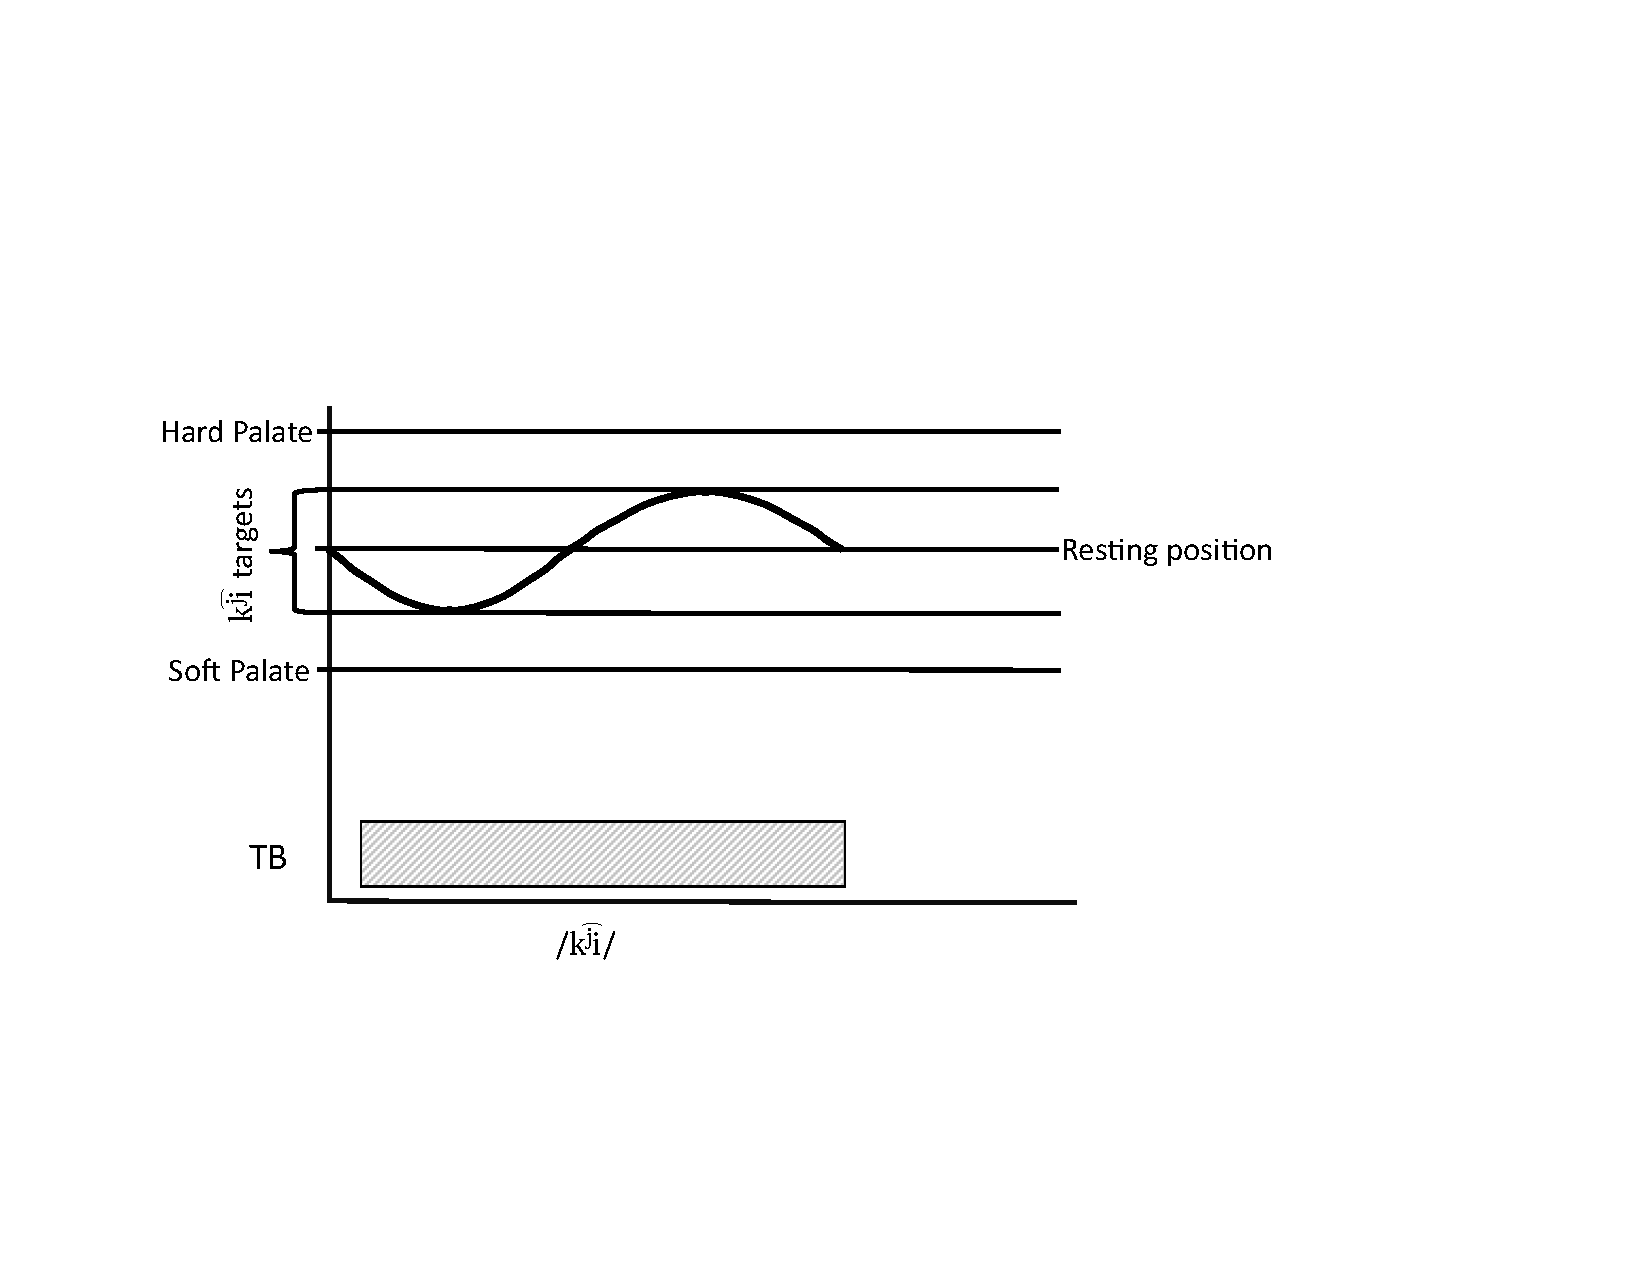
\includegraphics[width=.60\textwidth]{figures/palatalizationc.pdf}\caption{\label{fig:Palatalizationc}Possible production token derived from
perception token {[}{kʲi}{]}}
\end{figure}


\section{\label{subsec:Misperception-=000026-Misarticulation}Misperception \& misarticulation}

A well-established tradition in laboratory phonology attributes phonetic
and phonological sound change to mishearing and misspeaking on the
part of individual speakers and listeners \citep{Ohala1980,Ohala1981,ohala1983origin,Ohala1990}.
Many such changes are traced to coarticulation in production, which
can create perceptual ambiguity, and the possibility that what the
listener recovers is not what the speaker intended. In certain theories
of change, the rarity of sound change is attributed to the fact that
most speech takes place in a mode where speakers provide sufficient
cues for listeners, and listeners accurately reverse the effects of
coarticulation. Only rarely do listeners switch to a ``non-speech''
mode, in which they take the perceived forms at face value, or randomly
decide to keep a poor category exemplar, rather than discard it (e.g.
\citealp{lindblom1990explaining,Garrett2013}). In other theories,
discrepancies between speaker and listener are more common, and the
rarity of language-wide change is attributed to the listener's access
to other sources of information about the ``correct'' form of a word
(and/or the low likelihood of other speakers adopting and spreading
an individual's novel variant (e.g. \citealt{Ohala1980})). 

Perception biases emerge when segment \emph{x} is more likely to be
misheard as segment \emph{y}, than segment \emph{y} to be misheard
as segment \emph{x}. Production biases, in some cases, can be attributed
to the masking of overlapping articulatory gestures in rapid or casual
speech. These biases are of the same kind as those adopted in the
preceding models. Yet a fundamental aspect of the nature of these
misanalyses has been lost in implementation. Even in models that explicitly
invoke the Evolutionary Phonology framework (see \citealt{Blevins2004}),
the mechanism is typically realized at a very coarse grain.\footnote{Although \citet{Boer2000} uses a non-trivial mapping from acoustic
data to production targets, it is not a model of sound change, but
of structure emergence in vowel systems. In a similar type of model,
\citet{oudeyer2006self} relies on the same units (neurons) being
used in perception and production. However, this mapping is mediated
by the distributed nature of the representations (over a network of
neurons), and the fact that neurons are ``tuned'' by experienced input,
via a non-linear activation function. } For example, the model in \citet{wedel2017category} (also described
in \citet{Blevins2009}) is driven by misperception error (or “variant
trading”); this occurs as a binary decision between neighboring
lexical categories. As already discussed, \citet{Garrett2013} implement
an all-or-nothing normalization mechanism.\footnote{Although they make an explicit distinction between a word-level perceptual
token space, and a segment-level production token space, no transformation
algorithm is provided. They also suggest that the articulatory ``speech''
mode is sometimes available for perception, so the exact relationship
between the two ``modes'' of processing is somewhat unclear. In practice,
the models seem to be implemented using a single abstract phonetic
dimension.} In \citet{Kirby2014}, ``misparsing'' is more gradient; for any given
token, a random amount of the target segment may be mis-attributed
to the preceding segment. However, the misparsing doesn't depend on
the phonetic properties of the input, and different outcomes are only
possible by ``turning off'' the misparsing. \citet{morley2014implications}
uses a bi-directional misperception term in a model of velar palatalization,
but misperception only applies to feature parsing, and is segment
preserving. 

In the next chapter a new model of vowel nasalization is developed,
guided by the goal of avoiding the theoretical and implementational
pitfalls laid out in this, and preceding, chapters. This model will
contain an explicit listener analysis stage in which each token is parsed into its constituent units and the number of possible units is not fixed. Neither misparsing nor multiple processing modes is required because the input is not assumed to come pre-segmented at the phoneme level. Therefore, surface variation is directly reflected in underlying variation and change in one leads to change in the other.
